%% LaTeX-Beamer template for KIT design
%% by Erik Burger, Christian Hammer
%% title picture by Klaus Krogmann
%%
%% version 2.0
%%
%% mostly compatible to KIT corporate design v2.0
%% http://intranet.kit.edu/gestaltungsrichtlinien.php
%%
%% Problems, bugs and comments to
%% burger@kit.edu

\documentclass[18pt]{beamer}
\usetheme{kit}

%% TITLE PICTURE

% if a custom picture is to be used on the title page, copy it into the 'logos'
% directory, in the line below, replace 'mypicture' with the 
% filename (without extension) and uncomment the following line
% (picture proportions: 63 : 20, *.eps format if you use latex+dvips+ps2pdf,
% *.jpg/*.png/*.pdf if you use pdflatex)

%\titleimage{mypicture}

%% TITLE LOGO

% for a custom logo on the front page, copy your file into the 'logos'
% directory, insert the filename in the line below and uncomment it

%\titlelogo{mylogo}

% (*.eps format if you use latex+dvips+ps2pdf,
% *.jpg/*.png/*.pdf if you use pdflatex)

%% BIBTEX ICON/KEY

% if you want to see BibTeX keys in the references view instead of the symbol,
% uncomment the following line
% \usebibitemtemplate{\insertbiblabel}

% the presentation starts here

% change the following line to "ngerman" for German style date and logos
% change the following line to "english" for English style date and logos
\selectlanguage{ngerman}

\beamertemplatenavigationsymbolsempty

\usepackage{listings}
\definecolor{darkgray}{rgb}{0.95,0.95,0.95}
\definecolor{darkgreen}{rgb}{0.05,0.7,0.05}
\lstset{ language=Java,
	backgroundcolor=\color{darkgray}, 
	numbers=none, 
	keywordstyle=\color{black}\bfseries,
	tabsize=2,
	showspaces=false,               % show spaces adding particular underscores
	showstringspaces=false,         % underline spaces within strings
	showtabs=false, 
}



\title[Tutorium05]{Tutorium 05: Parallelismus und Testen}
\subtitle{Softwaretechnik im SS 2011, Tutorium 4}
\author{Jürgen Walter}
\date{\today}

\institute{Chair for Software Design and Quality}

\begin{document}

%title page
\begin{frame}
\titlepage
\end{frame}

%table of contents
\frame{
\frametitle{Was machen wir heute?}
	\tableofcontents
}

\section{Altes Übungsblatt}

\subsection{Altes Übungsblatt}
\frame {
\frametitle{Altes Übungsblatt}
	\begin{block}{Aufgabe 1 - Entwurfsmuster in der Java-API}
	\begin{itemize}
	\item ???
	\end{itemize}
	\end{block}

	\begin{block}{Aufgabe 2 - Kreuzworträtsel}
	\begin{itemize} \pause
	\item geschenkte Punkte \pause
	\item der Zusammenhang zwischen der Beschreibung und dem Muster sollte euch dennoch klar werden!
	\end{itemize}
	\end{block}
}


\begin{frame}[fragile]
\frametitle{Altes Übungsblatt}
	\begin{block}{Aufgabe 3 - Entwurfsmuster anwenden}
	\begin{itemize}
	\item ???
	\end{itemize}
	\end{block}
\end{frame}


\subsection{Zum Aufwärmen ...}
\frame {
\frametitle{Wahr oder falsch?}
\begin{itemize}
	\color<2->[rgb]{1,0,0}
	\item Die letzte Phase des klassischen Wasserfallmodells ist „Testen und Abnahme“.
	\color[rgb]{0,0,0}
	\pause
	\color<3->[rgb]{0,1,0}
	\item Regressionstests helfen verhindern, dass alte Fehler wieder auftreten.
	\color[rgb]{0,0,0}
	
	\pause
	\color<4->[rgb]{0,1,0}
	\item Eine Fabrikmethode kann eine Einschubmethode bei einer Schablonenmethode für Objekterzeugung sein.
	\color[rgb]{0,0,0}
	\pause
	\color<5->[rgb]{1,0,0}
	\item In Java muss eine Klasse, die eine Schnittstelle implementiert, alle in der Schnittstelle vorgegebenen Methoden implementieren
	\color[rgb]{0,0,0}
	\pause
	\color<6->[rgb]{1,0,0}
	\item In Java ist das Entwurfsmuster „Null-Objekt“ durch das Schüsselwort null realisiert.
	\color[rgb]{0,0,0}

\pause
	\color<7->[rgb]{0,1,0}
	\item Wenn eine Klasse eine abstrakte Methode besitzt, dann ist sie auch selbst abstrakt.
	\color[rgb]{0,0,0}

\pause
	\color<8->[rgb]{0,1,0}
	\item Zusicherungen (z.B. mit dem Schlüsselwort assert in Java) werden zur Laufzeit eines Programs ausgeführt und überprüft.
	\color[rgb]{0,0,0}
\end{itemize}
}

\frame {
\frametitle {Klausuraufgaben zum Aufwärmen} 
	\begin{block} {Aufgabe 1 (1P)}
Was ist der Nachteil von Zyklen in der Benutzt-Relation zwischen Modulen? \\
	\visible<2-> {
	Die einzelnen Module können nicht nacheinander implementiert
und getestet werden, weil ihr Funktionieren von einer korrekten
Implementierung aller Module des Zyklus abhängt. Oder:
„Nothing works until everything works.“
	}
	\end{block}
}

\frame {
\frametitle {Klausuraufgaben zum Aufwärmen} 
	\begin{block} {Aufgabe 2 (2P)}
Nennen Sie jeweils zwei in der Vorlesung besprochene Entwurfsmuster der Kategorien Entkopplungsmuster und Variantenmuster und ordnen Sie die genannten Entwurfsmuster der entsprechenden Kategorie zu. \\

	
	\begin{itemize}
		\item Entkopplungsmuster: 
		\visible<2-> {Adapter, Beobachter, Brücke, Iterator, Stellvertreter, Vermittler}
		\item Variantenmuster:
		\visible<3-> {Abstrakte Fabrik, Besucher, Erbauer, Fabrikmethode, Kompositum, Schablonenmethode, Strategie, Dekorierer}
	\end{itemize}
	
	\end{block}
}

\begin{frame}[fragile]
\frametitle {Klausuraufgaben zum Aufwärmen} 
	\begin{block} {Aufgabe 3 (1P)}

	\begin{lstlisting} {}
	public static double blub(double[] d) {
		if  (d != null \&\& d.length > 0) {
		...
		}
		...
	}
	\end{lstlisting}
	
	Begründen Sie: Was wäre die Folge, wenn man das \&\& durch ein \& ersetzt?
	\visible<2-> {
	Keine Kurzauswertung (0,5 P) 
	$\Rightarrow$ Bei null als Eingabe gäbe es eine NullPointerExeption bei d.length (0,5 P).
	}
	\end{block} 
\end{frame}

\section{Entwurfsmuster}

\frame{
\frametitle {Entwurfsmuster - Überblick}
	\begin{itemize}
		\item Entkopplungsmuster
		
		\begin{itemize}
			\item Adapter, Beobachter, Brücke, Iterator, Stellvertreter, Vermittler
		\end{itemize}
		
		\item Varianten-Muster
		\begin{itemize}
			\item Abstrakte Fabrik, Besucher, Fabrikmethode, Kompositum, Schablonenmethode, Strategie
		\end {itemize}
		\item Zustandshandhabungs-Muster
		\begin{itemize}
			\item Einzelstück, Fliegengewicht, Memento, Prototyp, Zustand
		\end{itemize}
		\item Steuerung-Muster
			\begin{itemize}
				\item Befehl, Master/Worker
			\end{itemize}
		\item Virtuelle Maschinen
		\item Bequemlichkeitsmuster
			\begin{itemize}
				\item Bequemlichkeits-Klasse, Bequemlichkeits-Methode, Fassade, Null-Objekt
			\end{itemize}
	\end{itemize}


}

\frame {
\frametitle {Klausuraufgabe 2006} 
	\begin{block} {Aufgabe (5)}
Ein binärer arithmetischer Ausdruck enthält einen Operanden, einen Operator (+ - * /) und einen anderen Operanden. Die Operanden können entweder eine Zahl sein oder selbst wieder ein anderer binärer arithmetischer Ausdruck. Entwerfen Sie mit Hilfe eines Entwurfsmusters ein Klassendiagramm, um die Bestandteile eines binären arithmetischen Ausdrucks zu einer Baumstruktur zusammenzufügen und seine Bestands-Hierarchien zu repräsentieren. Nennen Sie das verwendete Entwurfsmuster. Hinweis: z.B. 2 + 3 und (2 + 3) + (4 * 6) sind beide gültige arithmetische Ausdrücke. (5 P)
	\end{block} 

Welches Entwurfsmuster sollte man hier verwenden?
\visible<2-> {
	Kompositum
}
}


\frame {
\frametitle {Kompositum Allgemeines} 
	\begin{block} {Zweck}
	Füge Objekte zu Baumstrukturen zusammen, um Bestands-Hierarchien zu repräsentieren. Das Muster ermöglicht es 					Klienten, sowohl einzelne Objekte als auch Aggregate einheitlich zu behandeln.
	\end{block} 
	\begin{center}
		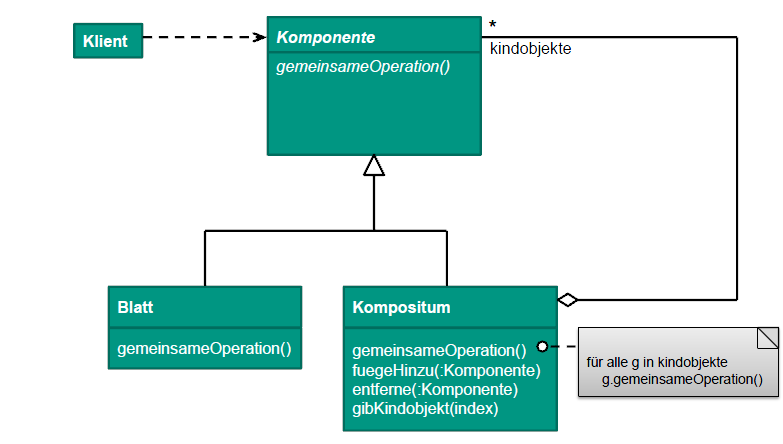
\includegraphics[scale=0.45]{pics/04/KompositumStruktur.png}
	\end{center}

}


\frame {
\frametitle{Zurück zur Aufgabe}
	\begin{block} {Aufgabe (5P)}
Ein binärer arithmetischer Ausdruck enthält einen Operanden, einen Operator (+ - * /) und einen anderen Operanden. Die Operanden können entweder eine Zahl sein oder selbst wieder ein anderer binärer arithmetischer Ausdruck. Entwerfen Sie mit Hilfe eines Entwurfsmusters ein Klassendiagramm, um die Bestandteile eines binären arithmetischen Ausdrucks zu einer Baumstruktur zusammenzufügen und seine Bestands-Hierarchien zu repräsentieren. Nennen Sie das verwendete Entwurfsmuster. Hinweis: z.B. 2 + 3 und (2 + 3) + (4 * 6) sind beide gültige arithmetische Ausdrücke. 
	\end{block} 
}

\frame {
\frametitle {Musterlösung}
	\begin{center}
		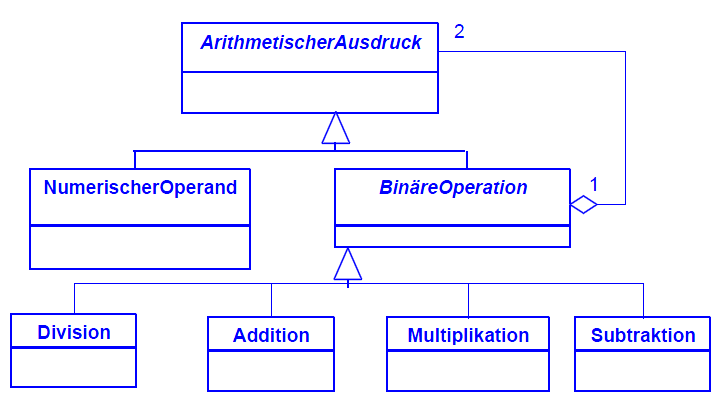
\includegraphics[scale=0.6]{pics/04/KompositumM.png}
	\end{center}
}

\frame {
\frametitle {Beobachter}
\begin{block} {Zweck}
Definiert eine 1-zu-n Abhängigkeit zwischen Objekten, so dass die Änderung eines Zustandes eines Objektes dazu führt, dass alle abhängigen Objekte benachrichtigt und automatisch aktualisiert werden.
\end{block}
\begin{center}
		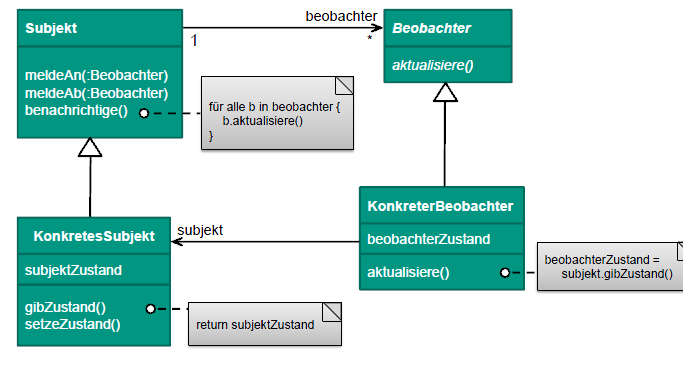
\includegraphics[scale=0.5]{pics/04/beobachter.png}
	\end{center}
}

\frame {
\frametitle {Brücke}
\begin{block} {Zweck}
Entkopple eine Abstraktion von ihrer Implementierung, so dass beide unabhängig voneinander variiert werden können.
\end{block}
	\begin{center}
		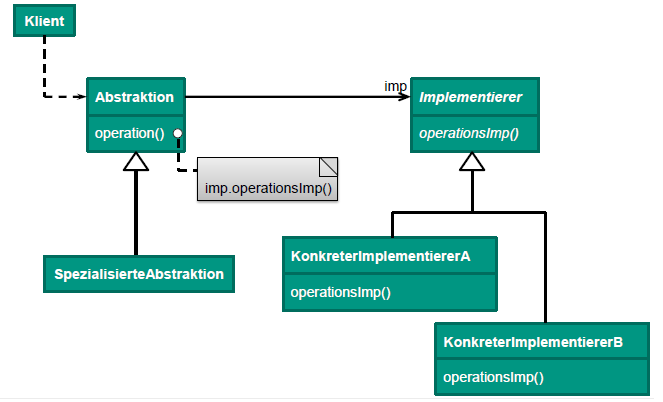
\includegraphics[scale=0.5]{pics/04/Bruecke.png}
	\end{center}
}

\frame {
\frametitle {Aufgabe: Brücke und Beobachter}

Der Begriff Shading bezeichnet in der 3D-Computergrafik im allgemeinen Sinne die Simulation der Oberfläche eines Objekts. Für die Berechnung der Oberfläche gibt es viele verschiedene Verfahren – unter anderem das Flat Shading und das Gouraud Shading. \\
\begin{wrapfigure}{r}{4cm}
	\centering
	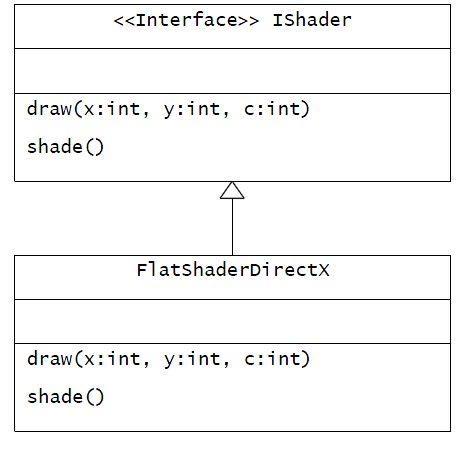
\includegraphics[scale=0.35]{pics/04/BrueckeA.png}
\end{wrapfigure}
Sie haben einen Flat Shader für die DirectX-Programmierschnittstelle entsprechend dem folgenden UML-Klassendiagramm entworfen.
Die Methode shade() in der Klasse FlatShaderDirectX implementiert den Flat Shading-Algorithmus und verwendet die Methode draw(x:int, y:int, c:int), um einen Punkt unter Verwendung der DirectX-Programmierschnittstelle zu zeichnen

}

\frame {
\frametitle {Aufgabe 1a - Brücke (7P)}
Verwenden Sie das Entwurfsmuster Brücke um die Abstraktion (Methode shade) von der Implementierung (Methode draw) zu trennen. \\
Hinweis: Trennen Sie die obige Schnittstelle IShader geeignet auf und erweitern Sie Ihr UML-Klassendiagramm um die konkreten Klassen DirectXImpl und OpenGLImpl, FlatShader und GouraudShader. Tragen Sie Vererbungsbeziehungen und Assoziationen entsprechend dem Entwurfsmuster Brücke ein. 
\begin{center}
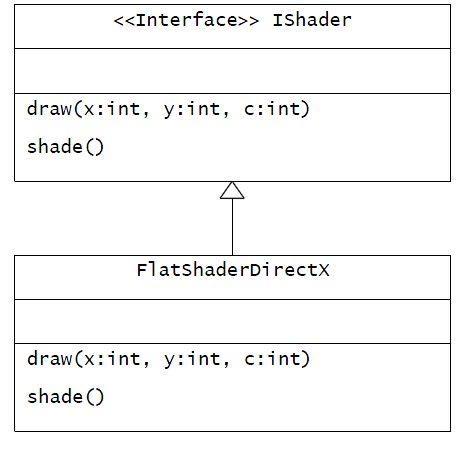
\includegraphics[scale=0.35]{pics/04/BrueckeA.png}
\end{center}
}


\frame {
\frametitle {Musterlösung  (7P)}
\begin{center}
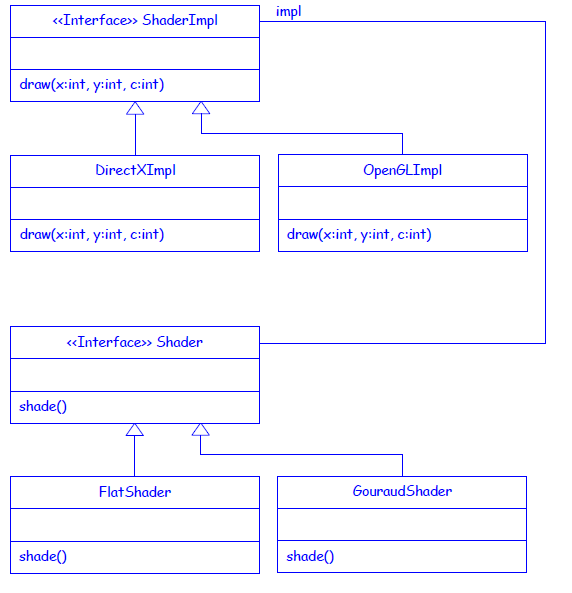
\includegraphics[scale=0.45]{pics/04/BrueckeM.png}
\end{center}
}

\frame {
\frametitle {Aufgabe 1b - Beobachter(3P)}
\small{Das Gittermodell, für das Ihre Shader-Klassen die Darstellungen der Oberflächen berechnen, wird von der Klasse Gittermodell verwaltet. Bei jeder Änderung des Git-termodells (Subjekt) soll der verwendete Shader (Beobachter) benachrichtigt werden. Verwenden Sie das Entwurfsmuster Beobachter und erweitern Sie das folgende UML-Klassendiagramm um Methoden-Signaturen für das An- und Abmelden, Benachrichtigen und Aktualisieren des Beobachters. \\
Hinweis: Definieren Sie keine zusätzlichen abstrakten Subjekt- und Beobachterklassen sondern verwenden und erweitern Sie lediglich die gegebene Schnittstelle Shader und die Klasse Gittermodell. 
}
\begin{center}
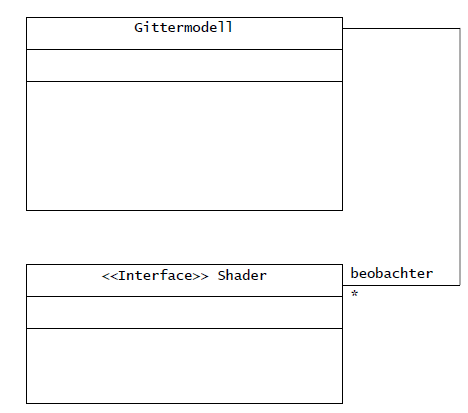
\includegraphics[scale=0.3]{pics/04/BeobachterA.png}
\end{center}
}


\frame {
\frametitle {Musterlösung}
\begin{center}
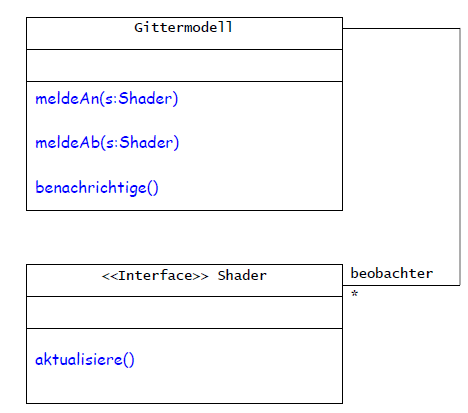
\includegraphics[scale=0.6]{pics/04/BeobachterM.png}
\end{center}
}

\frame {
\frametitle {Schablone}
\begin{block} {Zweck}
	\begin{itemize}
	\item Definiere das Skelett eines Algorithmus in einer Operation und delegiere einzelne Schritte an Unterklassen\\
		$\Rightarrow$ abstrakte Klasse die manche Details offen lässt
	\item ermöglicht es Unterklassen, bestimmte Schritte eines Algorithmus zu überschreiben, ohne seine Struktur zu verändern.
	\end{itemize}
\end{block}

	\begin{center}
		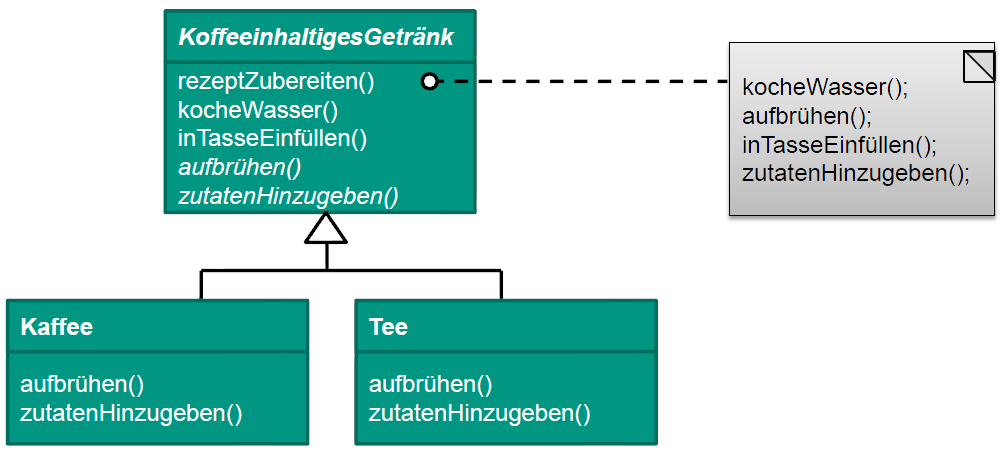
\includegraphics[scale=0.25]{pics/04/Schablone.png}
	\end{center}
}


\frame {
\frametitle {Strategie}
\begin{block} {Zweck}
	\begin{itemize}
	\item Definiere eine Familie von Algorithmen, kapsele sie und mache sie austauschbar.
	\item Ermöglicht es, den Algorithmus unabhängig von nutzenden Klienten zu variieren.
	\end{itemize}
\end{block}

	\begin{center}
		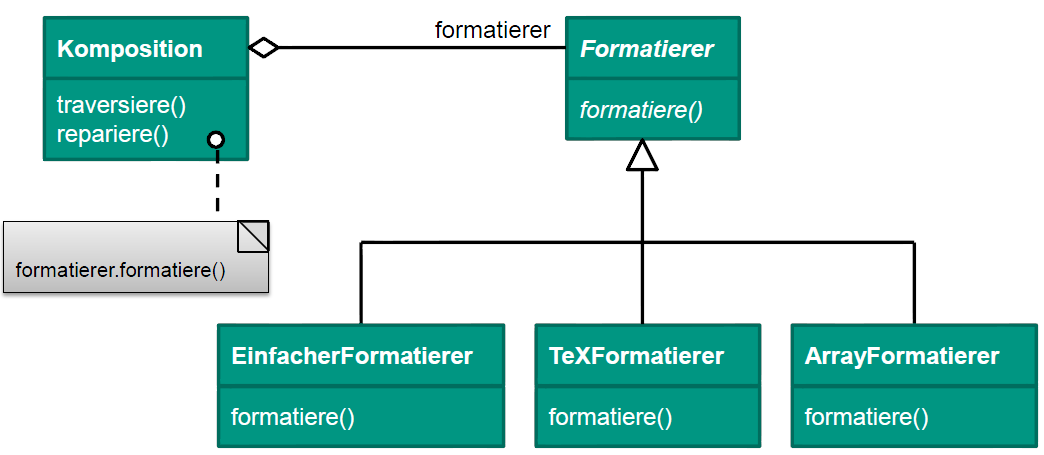
\includegraphics[scale=0.27]{pics/04/Strategie1.png}
	\end{center}
}

\frame {
\frametitle {Strategie}
\begin{block} {Zweck}
	\begin{itemize}
	\item Definiere eine Familie von Algorithmen, kapsele sie und mache sie austauschbar.
	\item Ermöglicht es, den Algorithmus unabhängig von nutzenden Klienten zu variieren.
	\end{itemize}
\end{block}

	\begin{center}
		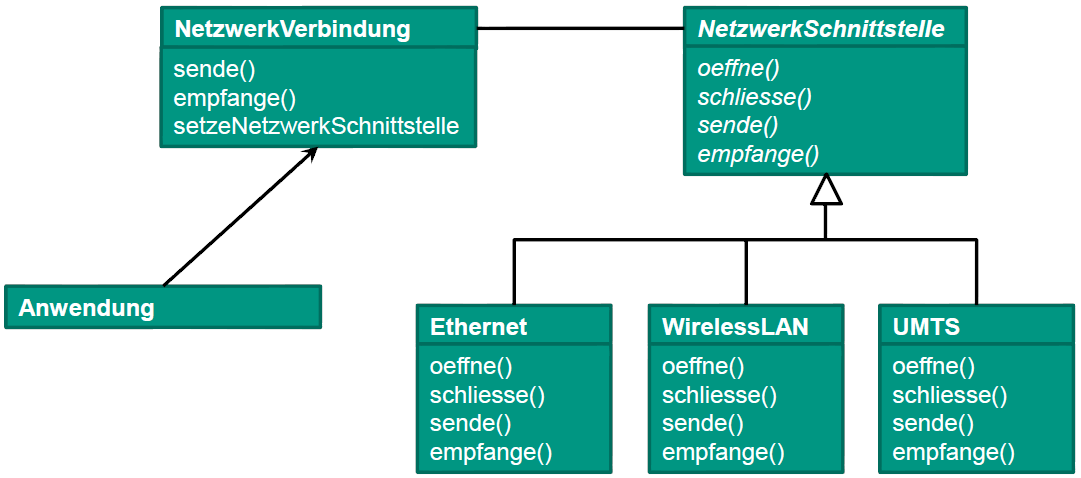
\includegraphics[scale=0.26]{pics/04/Strategie2.png}
	\end{center}
}

\frame {
\frametitle {Strategie vs. Schablone}
	\begin{block} {Gemeinsamkeit}
	\begin{itemize}
	\item beide sollen verschiedene Verhaltensvarianten ermöglichen
	\end{itemize}
\end{block} \pause

	\begin{block} {Unterschied}
	\begin{itemize}
	\item Strategie verwendet eine Aggregation von Implementierungen \pause
	\item Schablone wird i.d.R. während des Betriebs nicht ausgetauscht und ist nicht vom Aufrufer/Klienten getrennt.
	\end{itemize}
\end{block}
}

\frame {
\frametitle {Klausuraufgabe 2002}
\begin{block} {Fragen ...}
	\begin{itemize}
		\item Welches Entwurfsmuster sehen wir hier?		\visible<2-> {Schablonenmethode}
		\item Wie werden die Methoden 1, 2 und 3 genannt?  \visible<3-> {Einschubmethoden}
	\end{itemize}
\end{block}

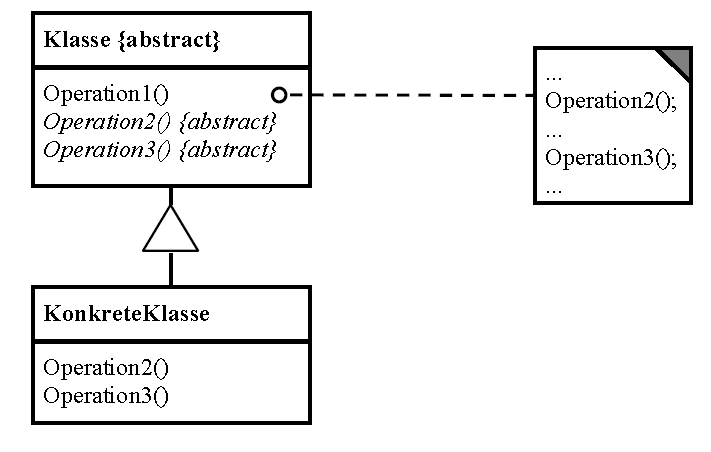
\includegraphics[scale=0.3]{pics/04/TemplateMethod.png}

}


\section{Kontrollflussorientiertes Testen}
\begin{block}{Aufgabe}
Gegeben sei der folgende Algorithmus, der Werte aus dem RGB-Farbraum in Werte des HSV-Farbraums umrechnet.
\begin{center}
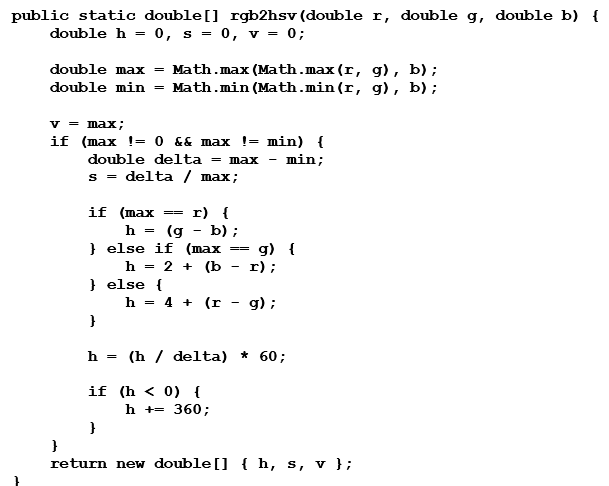
\includegraphics[scale=0.45]{pics/05/code.png}
\end{center}

a) Übersetzen sie den Algorithmus in die in der Vorlesung besprochene Zwischensprache und erstellen sie daraus den Kontrollflussgraphen

\end{block}
\section{Ende}
\subsection{Tipps zum nächsten Übungsblatt}

\frame{
\frametitle{Tipps zum nächsten Übungsblatt}

	\begin{block}{Aufgabe 1 - Kontrollflussorientiertes Testen}
	\begin{itemize}
	\item kommt oft in der Klausur vor \pause
	\item relativ leicht verdiente Punkte!
	\end{itemize}
	\end{block}
}

\frame{
\frametitle{Tipps zum nächsten Übungsblatt}

	\begin{block}{Aufgabe 2 -Gebietszerlegung und Synchronisation}
	\begin{itemize} \pause
	\item a) sollte jeder hinbekommen - falls euch nichts einfällt wählt einfach ein paar Parameter und schaut was passiert \pause
	\item b) sieht auf den ersten Blick harmlos aus - um sicher zu gehen programmiert ein Testprogramm und testet, ob euer Fix tatsächlich das Problem behebt \pause
	\item stellt dazu auch sicher, dass die ursprüngliche Barriere tatsächlich falsch funktioniert in eurem Test-Programm \pause
	\item ein Test ist nur dann sinnvoll, wenn er den Unterschied zwischen richtigem und falschem Code auch zeigt - \pause
	\item sonst kann es sein, dass euer Test das eigentliche Fehlverhalten nicht sichtbar macht
	\end{itemize}
	\end{block}
}


\frame{
\frametitle{Tipps zum nächsten Übungsblatt}
	\begin{block}{Aufgabe 3 - Parallelisierung}
	\begin{itemize}
	\item für diese Aufgabe gibt es 9 ``Pflicht''- und 5 Bonuspunkte
	\item ihr braucht zum Testen einen Rechner mit mindestens zwei Kernen - \\
		falls ihr keinen habt, gibt es in der Atis genug davon (Core2Duo, Core i5, Athlon X2)
	\item zuverlässige Laufzeitmessungen kann man oft brauchen, und es gibt dabei mehr als genug Fehlerquellen ;-)
	\end{itemize}
	\end{block}
}


\frame{
\frametitle{Bis zum nächsten Mal}
	\begin{center}
	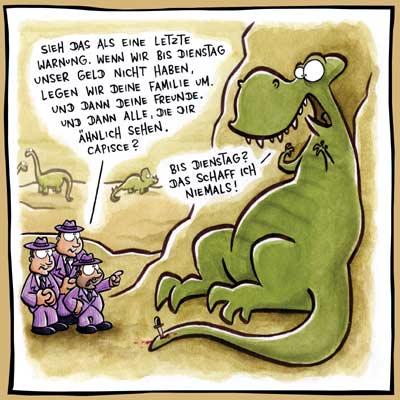
\includegraphics[height=200pt]{pics/05/05_comic}
	\end{center}
}

\end{document}
